% generated from src/4 Evaluation and privacy.md by tools/doc2tex.py; do not edit
\chapter{EVALUATION AND PRIVACY}

\section{Evaluation setup}

The system is evaluated at four levels: detection coverage, the per-student decision, the class estimate, and on-device performance. Several sources of evidence are used, because no single dataset has per-student attention labels for real lectures.

\textbf{System under test.} hcpose on a Raspberry Pi 5 with a Hailo-8 AI HAT (26 TOPS), Raspberry Pi OS trixie, HailoRT 4.23 / TAPPAS 5.1. The pose models are the project's own YOLOv8-pose upper-body models (13 keypoints) in three sizes, n, s and m, compiled to INT8 HEFs. Model weights were kept fixed throughout: all improvements are in pre- and post-processing and in the engagement logic.

\textbf{Evidence}

\begingroup\small
\begin{xltabular}{\textwidth}{*{4}{>{\raggedright\arraybackslash}X}}
\caption{Sources of evidence used in the evaluation}\label{tab:sources-of-evidence-used-in-the-evaluati}\\
\toprule
\textbf{Source} & \textbf{What it is} & \textbf{What it measures} & \textbf{Labels} \\
\midrule
\endfirsthead
\multicolumn{4}{l}{\emph{(continued)}}\\
\toprule
\textbf{Source} & \textbf{What it is} & \textbf{What it measures} & \textbf{Labels} \\
\midrule
\endhead
\bottomrule
\endlastfoot
SCB-Dataset (three subsets) \cite{b3} & 8,116 unique classroom images after merging duplicates, Chinese K-12 & detection coverage, per-student classifier accuracy (lesson-grouped 5-fold CV) & action boxes: read, write, hand-raising (focused); TurnHead, BowHead, discuss (distracted) \\
Exam-hall clip \cite{b17} & 72 s, high corner camera, about 30 adult students writing & false alarms, class estimate & none; context implies a share near 0 \\
Study-hall clip \cite{b18} & 6 min, camera at desk height, about 50 students & dense rooms, seat counting, low-camera failure & none; context implies a low share \\
Lecture clip \cite{b19} & 3 min 18 s, high front camera, about 35 students, mostly attentive & transfer of the classifiers to a real lecture & none; context implies a share near 0 \\
Small-class clip (clip\_5) & 14 min, iPhone mounted high at the front, 10 secondary-school students in three rows; a rough script the students did not consistently follow & false alarms and catches on a class nothing was tuned on; seat counting at close range & 150 student-moments labelled blind \\
Staged two-person session (clip\_4) & 4 min 45 s, phone mounted high at the front, two adults acting 7 scripted events & recall, precision, latency, false alarms during writing & exact per second, from the script \\
Human labels & 301 student-moments from two clips, labelled blind & precision and recall on real classes & focused / distracted / can't tell \\
\end{xltabular}
\endgroup

\textbf{Metrics.} Coverage = share of labelled students matched to a detection (centre coverage ≥ 0.5 or IoU ≥ 0.3). Per-student: AUC, within-image AUC (only images with both classes, which removes the ``recognise the image'' shortcut), balanced accuracy, precision and recall of \emph{distracted}. Class level: mean class distracted \%, the width of its 95\% range, and inferred class size. Device: FPS, latency, CPU, memory, temperature, throttling, power.

SCB numbers come from the deployed INT8 m HEF unless marked. Clip numbers come from the INT8 HEFs on the Pi; the two charts and the human-label scores use the same n model in FP32 on a PC, which the INT8 runs reproduce within a few points.

\section{Detection coverage and tiling}

Without tiling, the model misses most students in the far rows; running it again on three zoomed-in tiles of the top 60\% of the frame lifts coverage from 48.6\% to 75.5\% of labelled students at threshold 0.3, and from 17.0\% to 74.4\% in the far third.

\begin{figure}[htbp]
\centering
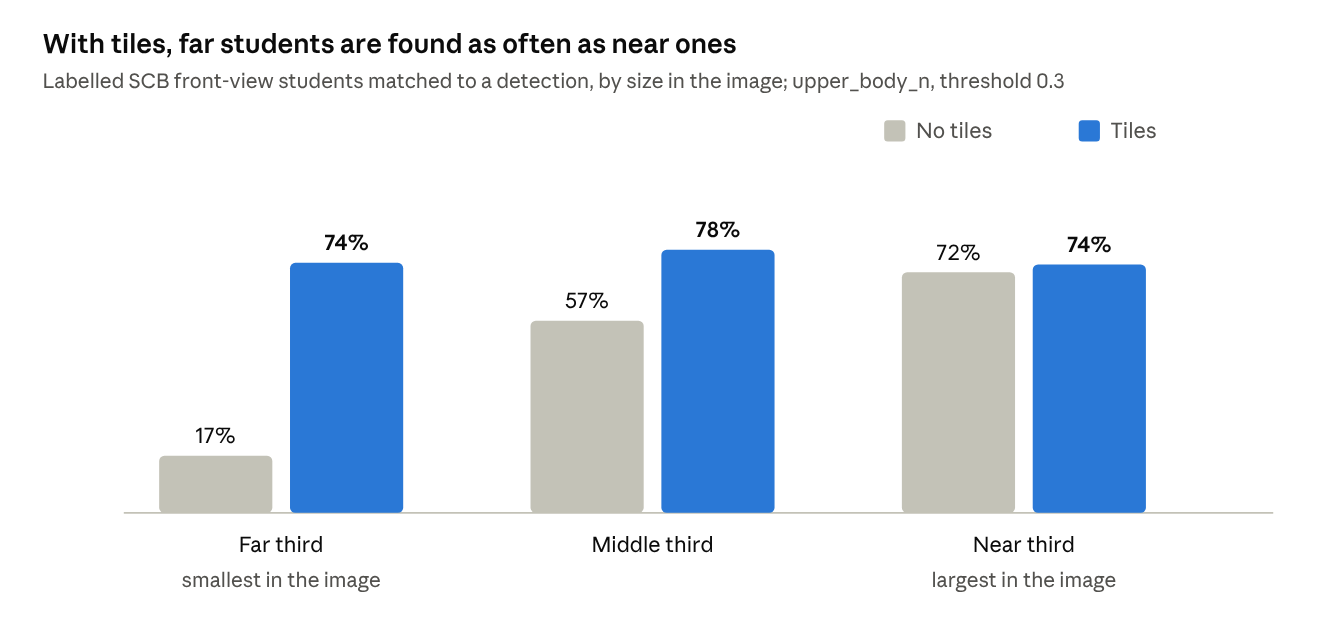
\includegraphics[width=0.75\textwidth]{figures/scb_coverage.png}
\caption{Labelled SCB front-view students detected, by size in the image, without and with tiles (upper\_body\_n, threshold 0.3)}\label{fig:labelled-scb-front-view-students-detecte}
\end{figure}

\textbf{Method.} Besides the full frame, the model runs on one row of overlapping, roughly square tiles over the top 60\% of the image (three tiles at 1280×720). Tile detections are mapped back to the frame; those cut by an inner tile edge are dropped, and duplicates across passes are merged by IoU, or by containment plus agreeing keypoints. Both engines implement the same rules; the C++ merge in the GStreamer pipeline was checked equal to the Python merge on 25 random scenes. The detector weights are unchanged.

\textbf{On the deployed INT8 m model}, the number of matched SCB front-view students rose from 23,186 without tiles to 36,226 with them (+56\%); 13,269 students were found only with tiles, 229 only without.

\textbf{On the classroom clips}, students per frame:

\begin{table}[htbp]\small
\caption{Students detected per frame on the classroom clips, without and with tiles}\label{tab:students-detected-per-frame-on-the-class}
\begin{tabularx}{\textwidth}{*{4}{>{\raggedright\arraybackslash}X}}
\toprule
\textbf{Clip} & \textbf{Model (INT8, Pi)} & \textbf{No tiles} & \textbf{Tiles} \\
\midrule
Exam hall & n & 12.6 & 18.6 \\
Exam hall & m & 14.2 & 22.1 \\
Lecture & n & 15.6 & 17.9 \\
Lecture & m & 20.1 & 22.0 \\
Study hall & n & 10.3 & 23.5 \\
Study hall & m & 10.6 & 21.0 \\
\bottomrule
\end{tabularx}
\end{table}

\textbf{Cost.} Full frame plus three tiles is four inferences per frame, and the frame rate drops by exactly four: n from 131 to 32.8 FPS (still real time) and m from 31.5 to 7.9 FPS (enough for engagement, which needs 5-10 FPS, but not for a live camera without dropping frames). The tiles help most in dense rooms with far rows, doubling the students found in the study hall; in the lecture clip, where the far rows are already large enough, they add only two to three per frame.

\section{Duplicate boxes and the class estimate}

Two post-processing fixes made the class-level number trustworthy: removing same-skeleton duplicate boxes, and counting only current, consistently seen seats. On the device, duplicates fell from 0.9-1.6 per frame to about 0.01, and the inferred class size now tracks the real head count.

\textbf{Same-skeleton duplicates.} YOLO-pose often outputs a tight and a loose box for one student with the same skeleton. Their box IoU is low, so box NMS keeps both, and the analyzer then counts one student twice. After NMS, a box is dropped when it lies inside a stronger box (≥ 70\% of the smaller box) and at least three keypoints visible in both are, on average, closer than 0.1 × √(smaller box area). The same rule runs in the NumPy and the C++ post-process.

\begin{table}[htbp]\small
\caption{Effect of same-skeleton duplicate removal}\label{tab:effect-of-same-skeleton-duplicate-remova}
\begin{tabularx}{\textwidth}{*{3}{>{\raggedright\arraybackslash}X}}
\toprule
\textbf{Measure} & \textbf{Before} & \textbf{After} \\
\midrule
SCB detections removed (1,500 images) & -- & 6.5\% (6.3\% with tiles) \\
Duplicate pairs per frame, exam clip, n, no tiles (Pi) & 1.63 & 0.01 \\
Duplicate pairs per frame, exam clip, m, tiles (Pi) & 1.54 & 0.00 \\
SCB coverage change & -- & −0.6 to −0.8 points \\
\bottomrule
\end{tabularx}
\end{table}

The small coverage loss is mostly the SCB matcher having credited a second student with the duplicate box.

\manualfigure{figures/manual/dedup}{A same-skeleton duplicate}{One student, two boxes on the same skeleton (left); after the same-skeleton check (right).}{fig:dedup}

\textbf{Class estimate.} A plain share of \emph{detected} students is biased, because missed students are mostly in the far rows and not missed at random. The estimate therefore:

\begin{enumerate}
\def\labelenumi{\arabic{enumi}.}
\tightlist
\item
  remembers each seat's last state for \texttt{presence\_seconds} (15 s), so a student missed for a few frames still counts;
\item
  splits the seats into near, middle and far zones by image height, and weights each zone by its number of seats rather than by how many students happen to be detected there;
\item
  counts a seat toward the class size only if it was seen in the last 60 s and, before calibration, in at least 15\% of frames;
\item
  puts a 95\% range around the shown (smoothed) estimate.
\end{enumerate}

The range is a Wilson score interval \cite{b16} for a share p measured on n of N students. With a known class size N (\texttt{-\/-class-size}), it is narrowed by the finite-population correction, shrinking toward p so p stays inside:

\begin{equation}
\tilde p = \frac{p + \frac{z^2}{2n}}{1 + \frac{z^2}{n}}, \qquad h = \frac{z}{1 + \frac{z^2}{n}} \sqrt{\frac{p(1-p)}{n} + \frac{z^2}{4n^2}}, \qquad f = \sqrt{\frac{N - n}{N - 1}}
\end{equation}

with z = 1.96; the range is {[}\ensuremath{\tilde{p}} − h, \ensuremath{\tilde{p}} + h{]} clipped to {[}0, 1{]}, and with a known N its ends move toward p by the factor f.~Without a known N, no correction is applied: a size inferred from the seats seen so far is itself a lower bound, so counting every known seat is not a census. The range covers students who weren't counted, not classifier mistakes.

\textbf{Seat counting.} Before step 3, every box that persisted about 1.5 s became a permanent seat. On the 6-minute study-hall clip the inferred class grew to 78 for about 50 students; with the rule it is 52, and 31 on the exam clip with about 30 students.

\textbf{Checks.} On the Pi, over 2,060 frames per setting, the shown estimate was never outside its range and the range was never zero-width. Without \texttt{-\/-class-size} the ranges are wide, 25-37 points for 20-30 counted students, which is honest for samples that small.

\section{Per-student decision: rules versus learned models}

The learned classifiers beat the rules on SCB by a wide margin, but on real classes they call attentive students distracted, so the rules are the system's default and the learned models are an opt-in comparison.

\textbf{The two approaches.} The rules combine pose cues with a noisy-OR: head yaw beyond the seat's calibrated baseline, head dropped below it, face hidden while the shoulders are visible, torso turned, a hand at the face; a raised hand always counts as focused. Each seat learns its own attentive pose in its first 120 s of observation, and labels are smoothed (EMA with hysteresis). The learned models (gradient-boosted trees, logistic regression, an MLP 64-32) take the keypoints and the same cues as features and are trained on SCB students with the deployed INT8 m model's poses, with and without tiles. They run in NumPy on the Pi.

\textbf{On SCB} (58,185 front-view students, 182 lessons, 5-fold cross-validation grouped by lesson):

\begin{table}[htbp]\small
\caption{Per-student decisions on SCB (lesson-grouped 5-fold cross-validation)}\label{tab:per-student-decisions-on-scb-lesson-grou}
\begin{tabularx}{\textwidth}{*{4}{>{\raggedright\arraybackslash}X}}
\toprule
\textbf{Decision} & \textbf{AUC} & \textbf{Within-image AUC} & \textbf{Balanced accuracy} \\
\midrule
Rules (single image, uncalibrated) & 0.55 & 0.54 & 56\% \\
Logistic regression & 0.772 & 0.735 & 71.3\% \\
Gradient-boosted trees & 0.855 & 0.840 & 77.0\% \\
MLP 64-32 & 0.863 & 0.838 & 78.0\% \\
\bottomrule
\end{tabularx}
\end{table}

The within-image AUC is the figure to quote: most SCB images contain only one class, so a model can partly recognise the image instead of the pose, and comparing students within the same image removes that shortcut. The rules are near chance here partly by design: they compare each student with their own calibrated pose, which a single image cannot provide.

\textbf{On real classes} the ranking reverses:

\begin{figure}[htbp]
\centering
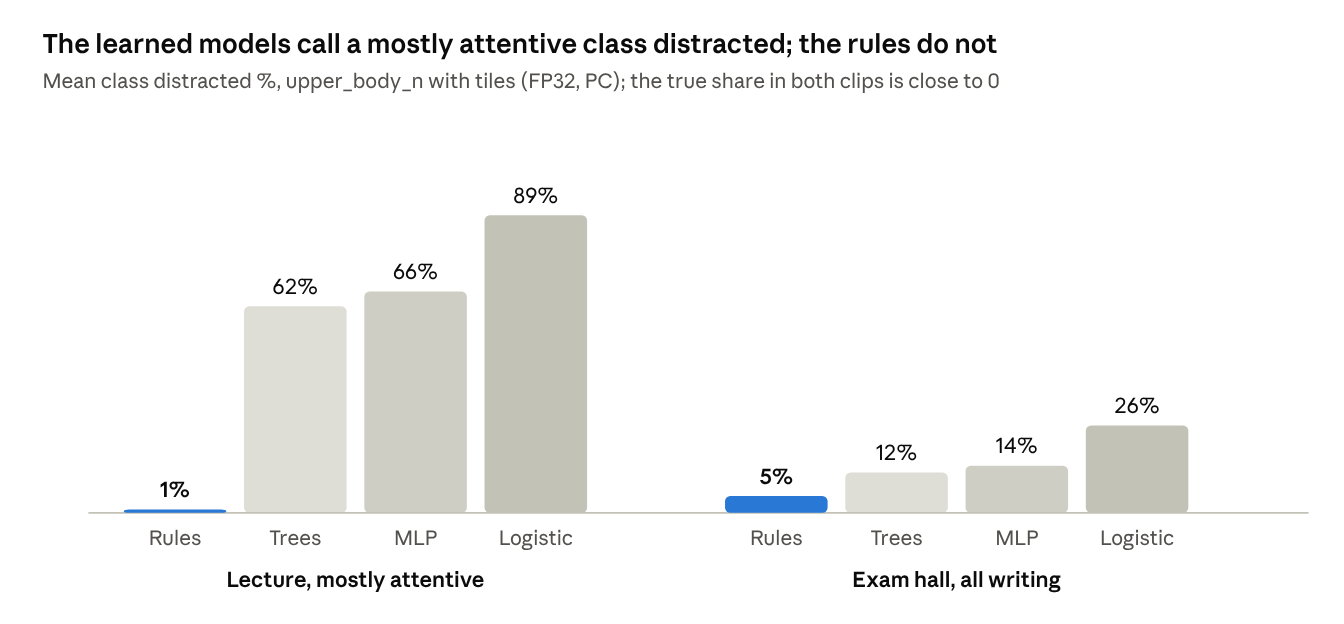
\includegraphics[width=0.75\textwidth]{figures/clips_rules_vs_learned.png}
\caption{Mean class distracted share on the lecture and exam-hall clips: rules against learned classifiers (upper\_body\_n with tiles, FP32)}\label{fig:mean-class-distracted-share-on-the-lectu}
\end{figure}

In the lecture clip, students sitting upright and looking at the board were labelled distracted, and students reading with their heads down focused (median head height above the shoulders 0.45 versus 0.32). The reason is a gap in SCB's labels: its focused classes are read, write and hand-raising, all head-down or hand-up, while its distracted classes include turning the head and discussing, both head-up. SCB has no ``listening'' or ``looking at the board'' label, the most common attentive state in a lecture, so a model trained on it learns that a raised head means distracted. Removing the head-height features did not fix it in a test, and the learned models also depend strongly on pose quality: with n and no tiles, trees gave 36\% on the exam clip on the Pi, against 9-13\% with m.

On the deployed INT8 models the picture is the same: in the lecture clip with m and tiles, the rules gave 0.0\% and the trees 48\%, logistic regression 74\% and the MLP 52\%.

\textbf{Against human labels.} 301 student-moments from the lecture and exam clips were labelled blind (focused, distracted or can't tell), sampled so that each disagreement between the rules and the trees was represented. Only 13 of the 275 judgeable moments (4.7\%) were distracted, 4.2\% when re-weighted to the whole clips. Pooled over both clips:

\begin{table}[htbp]\small
\caption{Per-student decisions against 301 blind human labels (lecture and exam-hall clips)}\label{tab:per-student-decisions-against-301-blind-}
\begin{tabularx}{\textwidth}{*{4}{>{\raggedright\arraybackslash}X}}
\toprule
\textbf{Decision} & \textbf{False alarms on focused moments} & \textbf{Specificity (95\% CI)} & \textbf{Distracted moments caught} \\
\midrule
Rules & 27 / 262 & 90\% (85-93\%) & 5 / 13 \\
Gradient-boosted trees & 114 / 262 & 56\% (50-62\%) & 3 / 13 \\
MLP 64-32 & 120 / 262 & 54\% (48-60\%) & 2 / 13 \\
Logistic regression & 199 / 262 & 24\% (19-30\%) & 5 / 13 \\
\bottomrule
\end{tabularx}
\end{table}

Re-weighted to the whole clips, the rules flag 1\% of lecture moments and 3\% of exam moments, close to the 4\% truth, while the learned models flag 56-94\% of lecture moments. Thirteen distracted moments are too few to estimate recall; the staged sessions measure it.

\textbf{Held-out class (clip\_5).} The deployment setting kept its low false-alarm rate on a class recorded after every threshold was fixed. 150 moments were labelled blind: 121 focused, 28 distracted and 1 can't tell, or 6.8\% distracted re-weighted to the whole clip. The moments were sampled from m-with-tiles detections, and a moment a run did not detect counts as not flagged. No frames of clip\_5 are shown, because its students are minors.

\begin{table}[htbp]\footnotesize
\caption{Per-student decisions against 150 blind human labels on the held-out class (clip\_5)}\label{tab:per-student-decisions-against-150-blind-}
\begin{tabularx}{\textwidth}{*{6}{>{\raggedright\arraybackslash}X}}
\toprule
\textbf{Model, tiles on} & \textbf{Decision} & \textbf{False alarms on focused} & \textbf{Specificity (95\% CI)} & \textbf{Distracted caught} & \textbf{Flagged share of the clip (re-weighted)} \\
\midrule
n & Rules & 11 / 121 & 91\% (84-95\%) & 8 / 28 & 4.7\% \\
n & Trees & 35 / 121 & 71\% (62-78\%) & 3 / 28 & 17.7\% \\
n & Logistic & 44 / 121 & 64\% (55-72\%) & 11 / 28 & 33.9\% \\
n & MLP & 42 / 121 & 65\% (56-73\%) & 9 / 28 & 28.4\% \\
m & Rules & 43 / 121 & 64\% (56-72\%) & 21 / 28 & 10.1\% \\
m & Trees & 51 / 121 & 58\% (49-66\%) & 12 / 28 & 11.4\% \\
m & Logistic & 55 / 121 & 55\% (46-63\%) & 10 / 28 & 35.4\% \\
m & MLP & 37 / 121 & 69\% (61-77\%) & 9 / 28 & 20.0\% \\
\bottomrule
\end{tabularx}
\end{table}

\begin{itemize}
\tightlist
\item
  \textbf{Rules on n:} 91\% specificity, against 90\% on the first label set. They flag 4.7\% of the clip against 6.8\% labelled, and catch 8 of 28 distracted moments.
\item
  \textbf{Learned models:} they again false-alarm far more, at 55-71\% specificity.
\item
  \textbf{Rules on m:} they catch the most (21 of 28) but flag 36\% of focused moments. Six of those 43 false alarms are on one front-row student.

  \begin{itemize}
  \tightlist
  \item
    The camera sees under that student's desk, so the box switches between upper body and full body. The models learned full-body boxes from COCO, whose person boxes cover the legs.
  \item
    The \texttt{body\_turned} cue divides shoulder width by box height, so the tall box reads as a turned torso.
  \end{itemize}
\item
  \textbf{Without tiles:} n leaves 92 of the 149 moments undetected.
\item
  \textbf{Seat counting:} with tiles, the analyzer found 13-17 seats for 10 students.

  \begin{itemize}
  \tightlist
  \item
    Seats are anchored at the top of the box. At this close range, a front-row head bending to write moves further than the seat-matching radius and opens a new seat.
  \item
    The full-body box adds a second seat on the same student.
  \item
    So after 2:30 the class indicator averages 11-15\% for the rules with tiles, against 6.8\% labelled.
  \end{itemize}
\end{itemize}

\textbf{Staged two-person session (clip\_4).} The author and a colleague, both adults, sat at one table filmed by a phone mounted high at the front, and followed a script for 4:45. Recording a script gives the true state of each person every second. After 55 s of attention, the script has seven distracted events:

\begin{itemize}
\tightlist
\item
  looking to the side (twice)
\item
  a phone under the table and a phone on the table
\item
  talking to each other
\item
  turning around
\end{itemize}

There is also a minute of writing, which should stay focused. Results on the INT8 m model (the n model in brackets where it differs):

\begin{table}[htbp]\small
\caption{Staged two-person session (clip\_4), INT8 m model}\label{tab:staged-two-person-session-clip-4-int8-m-}
\begin{tabularx}{\textwidth}{*{5}{>{\raggedright\arraybackslash}X}}
\toprule
\textbf{Decision} & \textbf{Distracted seconds caught} & \textbf{Precision} & \textbf{False alarms, attentive / writing} & \textbf{Events missed} \\
\midrule
Rules, original head-turn cue & 11\% & 100\% & 0\% / 0\% & 6 of 7 \\
Gradient-boosted trees & 40\% (17\%) & 100\% & 0\% / 0\% & 2 of 7 \\
MLP 64-32 & 40\% (11\%) & 100\% & 0\% / 0\% & 3 of 7 \\
Logistic regression & 34\% (19\%) & 64\% & 44\% / 0\% & 3 of 7 \\
Rules with the head-offset measure (new default) & 56\% (45\%) & 100\% & 0\% / 0\% & 2 of 7 \\
\bottomrule
\end{tabularx}
\end{table}

No decision caught the phone, whether on the table or under it. Head, wrists and elbows sit within about 0.2 shoulder-widths of where they sit when writing, so 13 upper-body keypoints cannot separate the two. The learned models' figures predate a seat-matching fix described below, so their turn-around seconds are slightly undercounted.

\textbf{Why the rules missed head turns.} The original head-turn cue measures yaw as the nose's position between the two ears. In profile the far ear disappears (confidence about 0.01), and the code falls back to estimating the head centre from the remaining ear. That ear has moved with the head, so the estimate cancels most of the turn:

\begin{table}[htbp]\small
\caption{Ear-based yaw and nose offset at attentive and turned moments of clip\_4}\label{tab:ear-based-yaw-and-nose-offset-at-attenti}
\begin{tabularx}{\textwidth}{*{4}{>{\raggedright\arraybackslash}X}}
\toprule
\textbf{Moment} & \textbf{Person} & \textbf{Ear-based yaw} & \textbf{Nose offset from the shoulder centre} \\
\midrule
Attentive & blue / grey & −0.15 / +0.07 & −0.07 / +0.05 \\
Talking to each other & grey & +0.03 & −0.35 \\
Looking to the side & blue & −0.31 (0.16 from his baseline) & −0.54 \\
\bottomrule
\end{tabularx}
\end{table}

The nose's offset from the shoulder centre, in shoulder-width units, shows every turn: about ±0.05 when attentive and ±0.35-0.54 when turned. It was added as a second head-turn measure, compared with each seat's own calibrated offset. The cue takes whichever of the two measures shows the larger turn. Like yaw, each seat's offset baseline is kept within 0.15 of the room's, so a student who looks away during calibration does not learn ``turned'' as attentive. The same session also showed that a student who turns around shrinks to a head-and-shoulders box whose centre jumps by about a third of its height, so seats are now anchored at the top of the box.

\textbf{Validation of the fix.} The offset's thresholds were chosen with clip\_4, so its clip\_4 recall is optimistic. Its cost was therefore measured on everything else, in a sweep over 16 settings on the saved INT8 skeletons. At the chosen ramp (0.2-0.4, other thresholds unchanged):

\begin{table}[htbp]\small
\caption{Effect of the head-offset measure across all evidence}\label{tab:effect-of-the-head-offset-measure-across}
\begin{tabularx}{\textwidth}{*{3}{>{\raggedright\arraybackslash}X}}
\toprule
\textbf{} & \textbf{n, before → after} & \textbf{m, before → after} \\
\midrule
clip\_4 distracted seconds caught & 11\% → 45\% & 11\% → 56\% \\
Human labels: false alarms on focused moments & 4\% → 5\% & 6\% → 7\% \\
Lecture class \% (truth near 0) & 4.7\% → 4.7\% & 0.0\% → 0.0\% \\
Exam-hall class \% & 3.6\% → 8.4\% & 11.7\% → 14.6\% \\
\bottomrule
\end{tabularx}
\end{table}

The only cost is 3-5 points on the exam clip. Some of that may be real, since the human labels found exam students looking around. Loosening the yaw thresholds alone reached only 25\% on clip\_4. The measure is now the default, and the 9-person session is kept as the held-out test.

The measure helps the rules only. The learned classifiers decide from the features they were trained on, which do not include it. It also cannot be learned from SCB: it needs a per-student baseline, and on SCB's single images with small faces it does not separate turned heads from reading (AUC 0.53).

\begin{figure}[htbp]
\centering
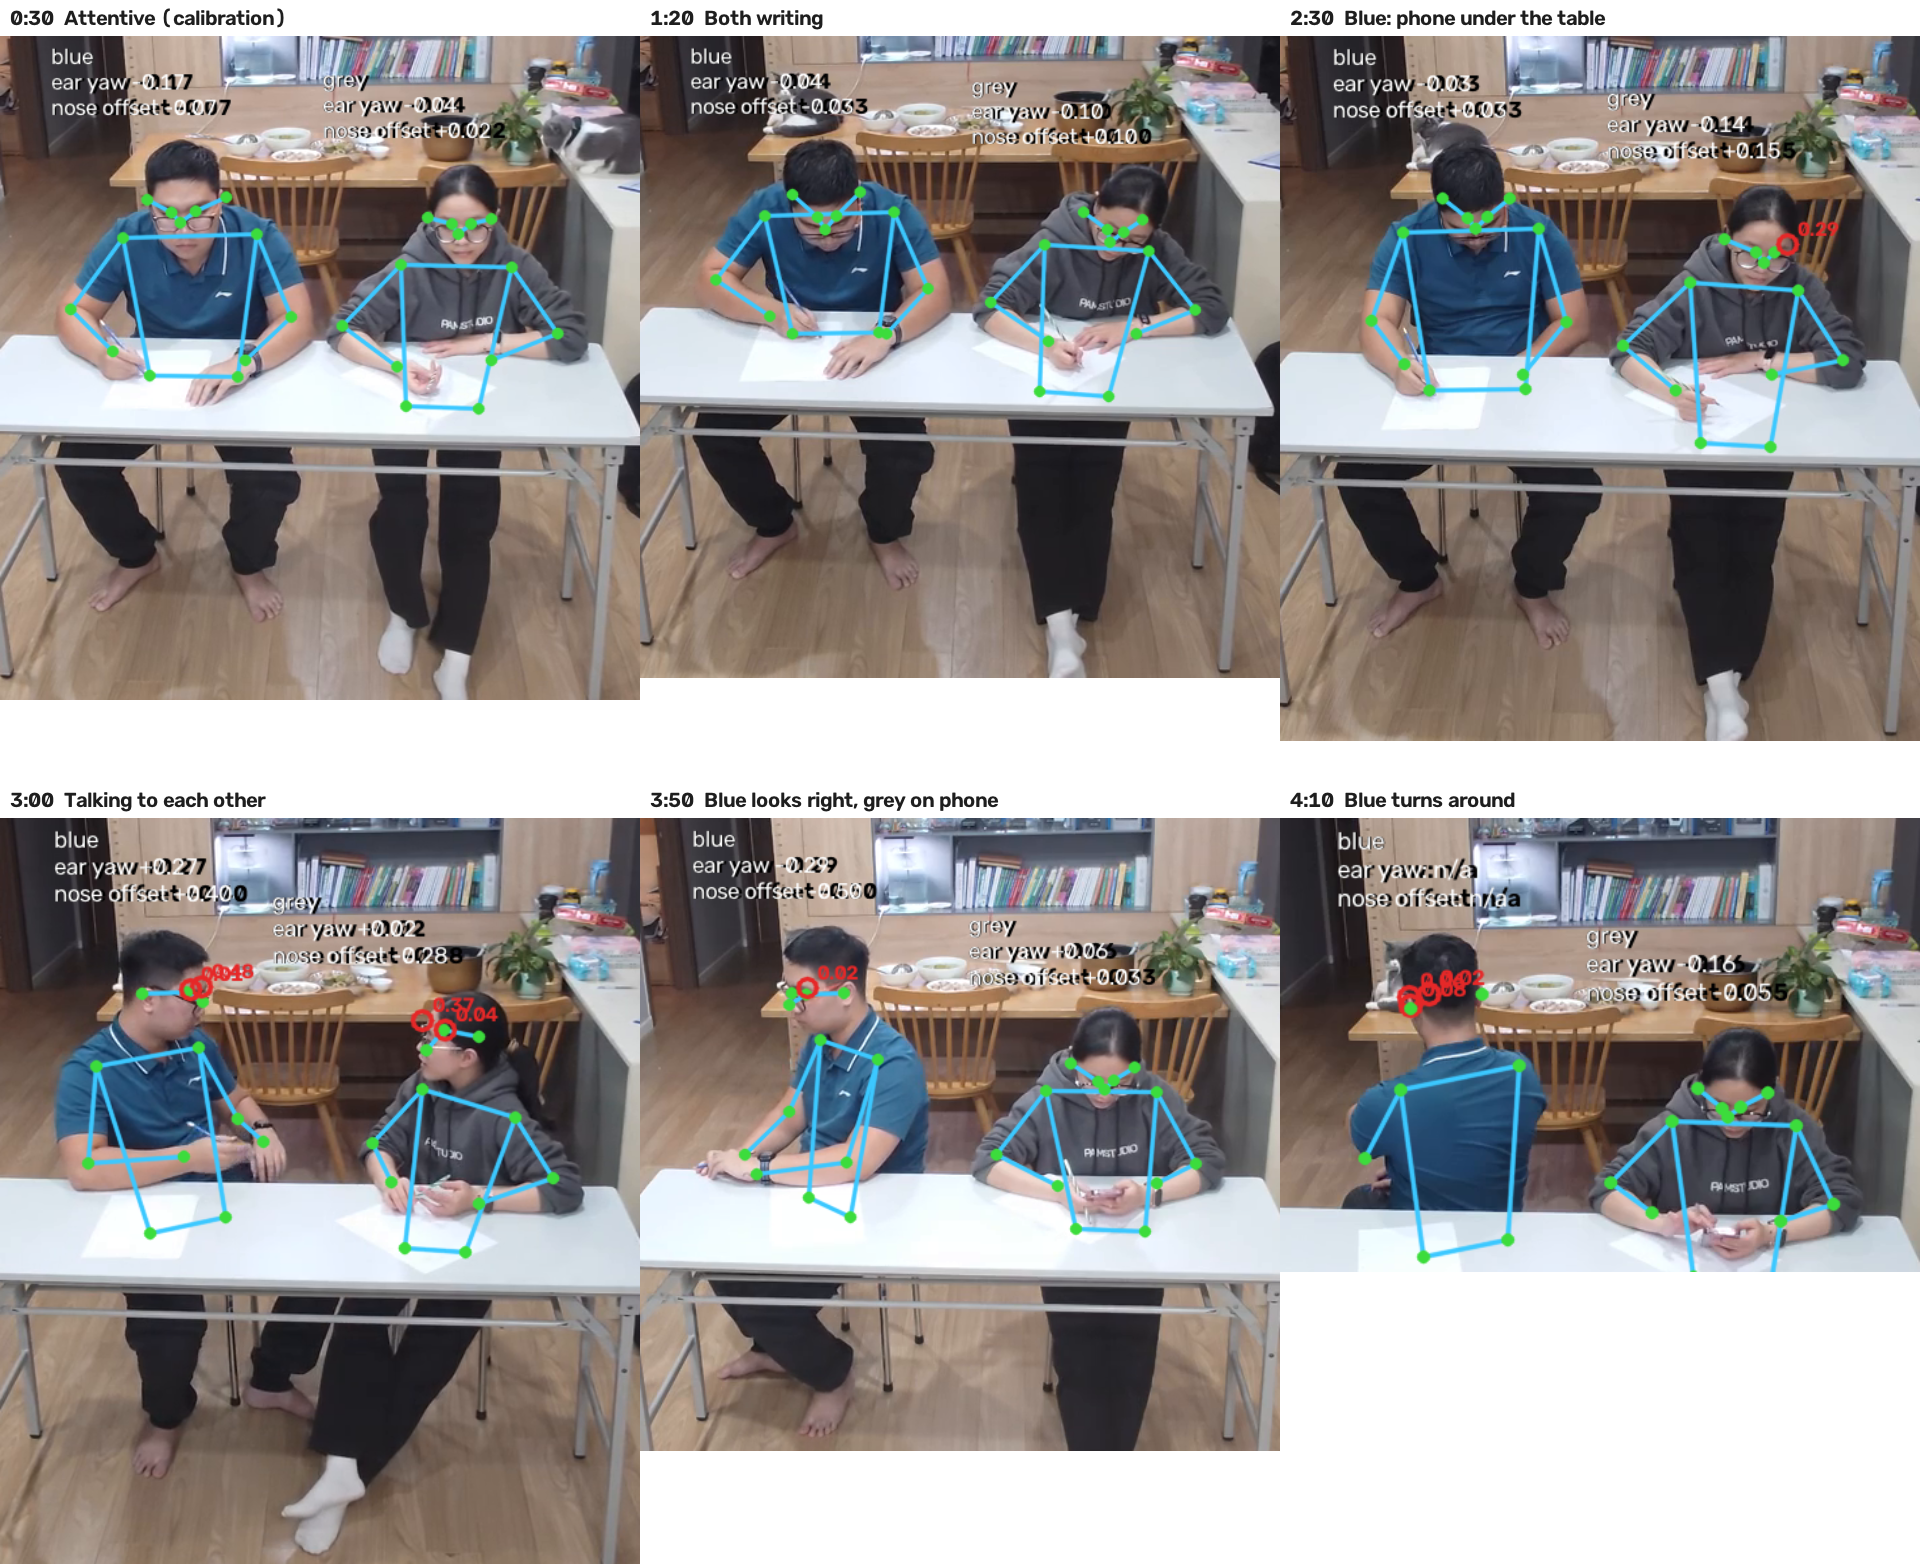
\includegraphics[width=1.0\textwidth]{figures/clip4_overview.png}
\caption{what the pose model sees on clip\_4, with the two head-turn measures per person}\label{fig:what-the-pose-model-sees-on-clip-4-with-}
\end{figure}

In profile the far ear's confidence falls to about 0.01, so the ear yaw reads near zero while the nose sits well to one side of the shoulders. The head-offset measure picks up these turns.

The benchmark accuracy of a classifier trained on a public action dataset therefore does not transfer to measuring attention; per-student calibration does better. Making a learned model usable would need training labels that include attentive, head-up students from the target classrooms, which the pending human labels and staged session begin to provide.

\section{Edge performance}

In the deployment setting, n with tiles in real time, the system ran for 15 minutes at 30 FPS with 45 ms latency, 4.3 W measured on the Pi board plus 2.5 W for the Hailo-8 (vendor figure), a peak SoC temperature of 60 °C and no throttling. The pipeline is bound by the Hailo-8, not the CPU. All figures below were measured on the Pi 5 with official Raspberry Pi active cooling on its fan header, on 10 November 2026.

\textbf{Hailo-8 alone} (\texttt{hailortcli\ benchmark}, INT8 HEFs):

\begin{table}[htbp]\small
\caption{Hailo-8 throughput and latency per model (hailortcli benchmark)}\label{tab:hailo-8-throughput-and-latency-per-model}
\begin{tabularx}{\textwidth}{*{3}{>{\raggedright\arraybackslash}X}}
\toprule
\textbf{Model} & \textbf{FPS} & \textbf{Hardware latency (ms)} \\
\midrule
n & 131.5 & 5.7 \\
s & 69.5 & 11.9 \\
m & 31.5 & 26.7 \\
\bottomrule
\end{tabularx}
\end{table}

\textbf{End to end} (lecture clip, 1280×720, GStreamer engine, engagement on, as fast as possible):

\begin{table}[htbp]\footnotesize
\caption{End-to-end performance on the Raspberry Pi 5 (lecture clip, 1280×720)}\label{tab:end-to-end-performance-on-the-raspberry-}
\begin{tabularx}{\textwidth}{*{7}{>{\raggedright\arraybackslash}X}}
\toprule
\textbf{Model} & \textbf{Tiles} & \textbf{FPS} & \textbf{CPU, whole Pi} & \textbf{Memory of hcpose (MB)} & \textbf{Max SoC temp (°C)} & \textbf{Pi board power (W)} \\
\midrule
n & off & 119.1 & 79\% & 332 & 61.1 & 5.42 \\
n & on & 32.8 & 46\% & 286 & 60.6 & 4.84 \\
s & off & 69.3 & 47\% & 329 & 60.1 & 4.77 \\
s & on & 17.4 & 26\% & 294 & 59.5 & 3.87 \\
m & off & 31.5 & 23\% & 339 & 58.4 & 3.19 \\
m & on & 7.9 & 14\% & 307 & 57.3 & 2.82 \\
\bottomrule
\end{tabularx}
\end{table}

End-to-end FPS matches the Hailo-only figures, and four passes per frame divide them by exactly four. The CPU's main cost is the engagement analysis, about 2.8 cores at 119 FPS. Board power is lower for the slower settings because the Pi waits on the accelerator.

\textbf{Latency.} Frames were released at the clip's 25 FPS, as a camera releases them, and timed from that point to the sink with GstShark's interlatency tracer \cite{b20}: median 20 ms for n (95th percentile 23), 45 ms for n with tiles (53), and 40 ms for m (47). m with tiles cannot keep up with a 25 FPS camera (7.9 FPS): frames queue and latency settles at 2.5 s, so a live m-with-tiles deployment needs a leaky queue or a lower camera rate.

\textbf{Thermal behaviour} over two 15-minute runs:

\begin{table}[htbp]\footnotesize
\caption{Thermal behaviour over 15-minute runs}\label{tab:thermal-behaviour-over-15-minute-runs}
\begin{tabularx}{\textwidth}{*{6}{>{\raggedright\arraybackslash}X}}
\toprule
\textbf{Run} & \textbf{FPS} & \textbf{SoC temperature after 5 / 10 / 15 min (°C)} & \textbf{Max (°C)} & \textbf{Throttling} & \textbf{Pi board power (W)} \\
\midrule
n with tiles, real time (deployment) & 30.0 & 56.8 / 57.9 / 56.8 & 60.1 & none & 4.26 \\
m with tiles, as fast as possible & 7.9 & 53.5 / 55.6 / 54.6 & 56.2 & none & 2.70 \\
\bottomrule
\end{tabularx}
\end{table}

Idle, the Pi drew 2.33 W at 50 °C.

\textbf{Power.} Board power is the sum of voltage × current over the Pi 5's PMIC rails (\texttt{vcgencmd\ pmic\_read\_adc}). It excludes the AI HAT and USB devices, so the Hailo-8 is added from vendor figures:

\begin{table}[htbp]\small
\caption{Vendor power figures used to complete the measured board power}\label{tab:vendor-power-figures-used-to-complete-th}
\begin{tabularx}{\textwidth}{*{3}{>{\raggedright\arraybackslash}X}}
\toprule
\textbf{Part} & \textbf{Figure} & \textbf{Source} \\
\midrule
Raspberry Pi 5, typical bare-board active current & 800 mA at 5 V ≈ 4 W & \href{https://www.raspberrypi.com/documentation/computers/raspberry-pi.html\#power-supply}{Raspberry Pi documentation} \cite{b21} \\
Raspberry Pi 5, recommended supply & 5 V, 5 A (27 W) & same \\
Hailo-8, typical power & 2.5 W & \href{https://hailo.ai/products/ai-accelerators/hailo-8-ai-accelerator/}{Hailo} \cite{b5} \\
Hailo-8 M.2 module, maximum & 8.65 W & \href{https://core-electronics.com.au/hailo-8-m2-ai-accelerator-module-26-tops.html}{Core Electronics listing} \cite{b22} \\
AI HAT+, operating ambient & 0-50 °C & \href{https://cdn.sparkfun.com/assets/c/9/b/7/3/Raspberry_Pi_AI_HAT__product_brief.pdf}{AI HAT+ product brief} \cite{b23} \\
\bottomrule
\end{tabularx}
\end{table}

The deployment setting therefore draws about 4.3 W (measured) + 2.5 W (typical, vendor) ≈ 6.8 W, well within one 27 W USB-C supply. The measured board figure agrees with the vendor's 4 W typical. 26 TOPS at 2.5 W is about 10 TOPS/W (own calculation from Hailo's figures).

\section{Privacy by design}

The system never stores or transmits an image by default: each frame lives in memory for one inference, and the only default output is a class-level share shown on the teacher's screen.

\begin{figure}[htbp]
\centering
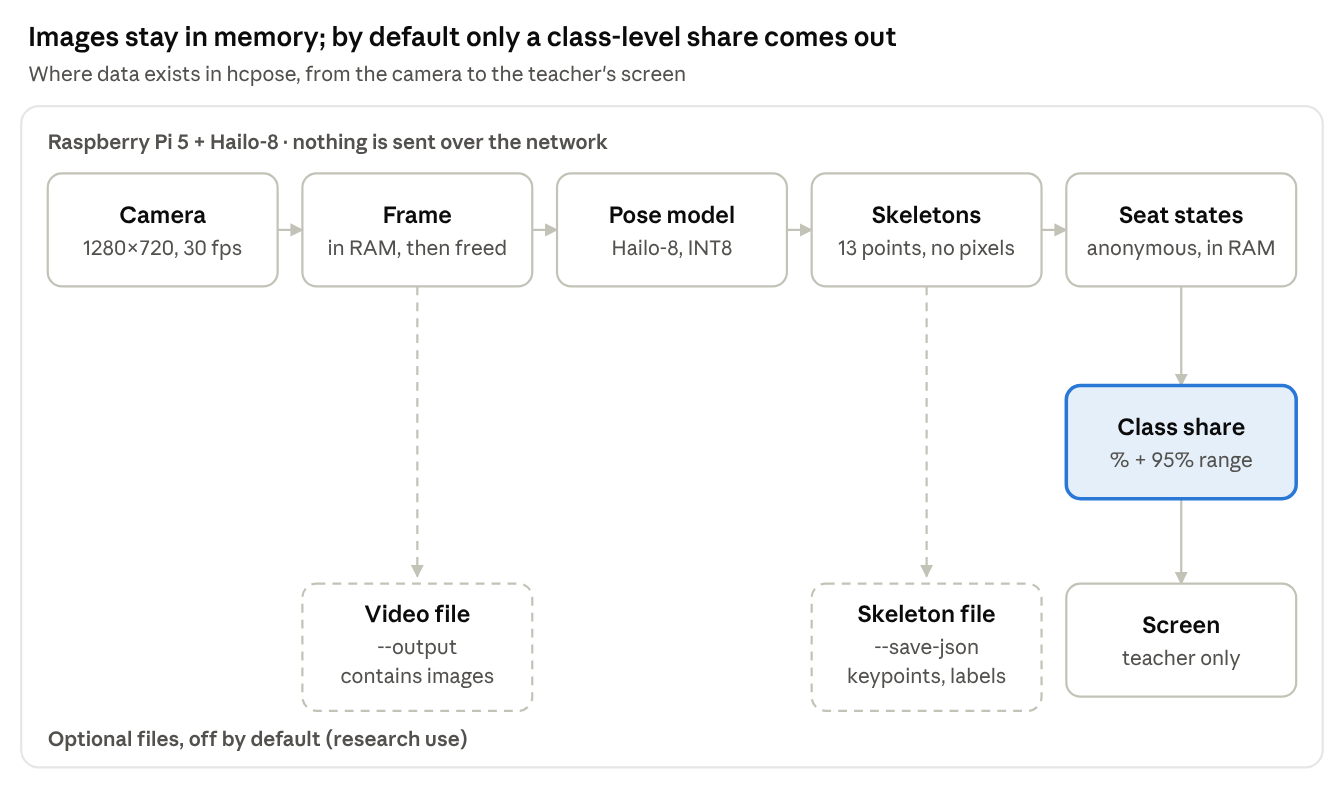
\includegraphics[width=0.9\textwidth]{figures/dataflow.png}
\caption{Data flow in hcpose with default settings; optional outputs are dashed}\label{fig:data-flow-in-hcpose-with-default-setting}
\end{figure}

\begin{itemize}
\tightlist
\item
  \textbf{Frames} are decoded into RAM, passed to the Hailo-8 and freed. Nothing is written to disk unless \texttt{-\/-output} is set, which is meant for development and evaluation, not for classes.
\item
  \textbf{Skeletons} (13 keypoints and a box per person) carry no pixels. They identify nobody by themselves, but tied to a seat and a time in a known class they could point to a student, so they are treated as personal data and kept in memory.
\item
  \textbf{Seat states} use anonymous seat numbers that exist only for one session. There is no face recognition, no name list and no link between sessions, except an optional calibration file (\texttt{-\/-calibration}) that stores each seat's attentive pose and position, not identities.
\item
  \textbf{The class share} with its range is the only number meant to leave the program. It describes the class, not a student, and is not personal data.
\item
  \textbf{The screen} shows the camera image with labels during development. For classroom use, \texttt{-\/-display\ class} limits the overlay to the class number, and \texttt{-\/-headless} shows no window at all.
\item
  \textbf{Network:} hcpose opens no network connection; the device can run fully offline.
\end{itemize}

What a saved record holds, when \texttt{-\/-save-json} is used: one line per frame, from clip\_4 at 3:50, shortened to one person and three of the 13 keypoints. There are coordinates, scores and states, but no pixels and no identity. The seat number exists only within the session.

\begin{codeblock}
{"type": "frame", "t": 229.97, "w": 1280, "h": 720,
 "class": {"visible": 2, "counted": 2, "focused": 1, "distracted": 1,
           "class_pct_distracted": 33.3, "class_ci": [6.1, 79.2], "class_size": 3},
 "persons": [{"score": 0.75, "box": [663.9, 296.1, 863.6, 709.2],
              "keypoints": [[771.9, 356.1, 0.98], [776.5, 348.7, 0.91], [761.6, 349.6, 0.95], "…"],
              "engagement": {"seat": 2, "state": "focused", "score": 0.0, "reason": null, "calibrated": true}}]}
\end{codeblock}

Compared with a cloud service, nothing has to be uploaded, stored by a third party or transferred across borders, which removes the cross-border transfer obligations and most of the breach risk.

\section{Legal fit in Vietnam}

Since 1 January 2026, personal data in Vietnam is governed by the Law on Personal Data Protection (No.~91/2025/QH15) \cite{b12} and its implementing Decree 356/2025/ND-CP, which replaced Decree 13/2023/ND-CP. Keeping video on the device and reporting a class-level share lowers, but does not remove, the obligations of a school using the system. This section is an analysis for the thesis, not legal advice.

\begingroup\small
\begin{xltabular}{\textwidth}{*{3}{>{\raggedright\arraybackslash}X}}
\caption{Provisions of Law 91/2025/QH15 and Decree 356/2025/ND-CP and their consequences for the system}\label{tab:provisions-of-law-91-2025-qh15-and-decre}\\
\toprule
\textbf{Provision} & \textbf{What it says} & \textbf{Consequence for the system} \\
\midrule
\endfirsthead
\multicolumn{3}{l}{\emph{(continued)}}\\
\toprule
\textbf{Provision} & \textbf{What it says} & \textbf{Consequence for the system} \\
\midrule
\endhead
\bottomrule
\endlastfoot
Personal data (Law, Art. 2.1) & data that ``identifies or helps identify a specific person'' & Camera frames are personal data. Keypoints tied to a seat and a time in a known class can help identify a student, so per-student skeletons and labels are treated as personal data too; the class-level share is not. \\
Sensitive data (Law, Art. 2.3; Decree 356, Art. 4) & data tied to privacy, on a Government list that includes biometric data & hcpose does no face recognition and keeps no identity. Whether body keypoints for behaviour analysis count as biometric is not settled, so the design treats per-student data as if it were sensitive: kept in memory by default, never transmitted. \\
Purpose limitation (Law, Art. 3.2) & processing ``for specific and clear purposes'' & One stated purpose: an aggregate attention indicator for the teacher. No per-student report, ranking or grading. \\
Consent (Law; Decree 356, Art. 9) & consent per purpose; no default or bundled consent & The school informs students and parents and obtains consent for the camera and this purpose before deployment. \\
Children (Law, Art. 24.2) & legal representatives act for children; children aged 7 or older must also consent where their private life is disclosed & Most pupils are minors: parental consent is needed, and older pupils should be informed and asked as well. \\
Recording in public places (Law, Art. 32) & allowed without consent only for listed public activities, with notice & A classroom lesson is not one of the listed cases, so the consent route above applies. \\
Impact assessment (Law; Decree 356) & a processing impact assessment, updated when processing changes & A school deploying it prepares a DPIA. The small-business grace period does not cover processing sensitive data directly. \\
Breach notification & within 72 hours & With nothing stored by default there is little to breach; any saved files fall under it. \\
\end{xltabular}
\endgroup

\textbf{What the design contributes.} Data minimisation and storage limitation are built in: frames exist only in RAM for the time of one inference, nothing leaves the device, and the default output is a class-level number. What stays the school's job: notice, consent, a DPIA, and keeping the optional research outputs (annotated video, skeleton files) switched off in live use.

Sources: \cite{b12,b24,b25,b26,b27}. Article numbers follow the English translation; check them against the official Vietnamese text before citing.

\section{Limitations and threats to validity}

The largest gap is ground truth: no result so far measures per-student accuracy on a real lecture, only on SCB actions or through the context of mostly attentive clips.

\begin{itemize}
\tightlist
\item
  \textbf{Proxy labels.} SCB labels actions (reading, turning, discussing), not attention, and comes mostly from Chinese K-12 classrooms. About 2,000 SCB students carried both a focused and a distracted label across duplicate images, mostly ``bowed head'' versus ``reading or writing'', so even the annotators could not separate these.
\item
  \textbf{Clip evidence is contextual.} The three clips have no labels; ``the true share is close to 0'' rests on what the class is doing. They show false alarms, not missed distraction. The human labels and the staged session address this.
\item
  \textbf{Few rooms, third-party footage.} Three third-party clips from three rooms, one of them with a camera outside the intended mounting, plus one small class recorded for this work. Results may not carry over to other layouts, lighting or age groups.
\item
  \textbf{Camera height.} With a camera at desk height, a head bowed over writing hides the face and reads as ``turned away'': the rules gave 44\% distracted in a study hall where everyone wrote. The design assumes a camera mounted high at the front; a lower \texttt{face\_hidden} weight (0.3) halves the error for low cameras.
\item
  \textbf{Calibration time.} Each seat needs 120 s of usable observation. In a 6-minute dense clip only 20 of 52 seats finished calibrating, so short sessions run mostly on room-level baselines.
\item
  \textbf{Small classes, wide ranges.} With 20-30 counted students the 95\% range spans 25-37 points unless the head count is given. This is a property of the sample size, not a defect, but it limits how finely the indicator can be read.
\item
  \textbf{Hand-set rule weights.} The rule weights were set by design, not fitted, and were deliberately not tuned on the clips used to evaluate them; one documented change, the low-camera weight, is an option rather than the default.
\item
  \textbf{Mixed precision of the evidence.} The two charts and the human-label scores use the n model in FP32 on a PC; the INT8 runs on the Pi reproduce the class-level numbers within a few points. m with tiles also cannot keep up with a live 25-30 FPS camera without dropping frames.
\item
  \textbf{Staged session.} Adult volunteers acting scripted behaviour in a small room are easier to see and more exaggerated than real distraction, so its recall is an upper bound.
\item
  \textbf{Close cameras and full-body boxes.} In a small room filmed from close range, seats multiply (13-17 for 10 students in clip\_5), and a full-body box on a student whose legs are visible reads as a turned torso. Both come from geometry tied to the box: the seat anchor at its top and the box height in \texttt{body\_turned}. Keypoint-based anchors and scales would avoid them; they were not changed after clip\_5, to keep it a held-out test.
\end{itemize}
